\documentclass{beamer}
\usepackage[utf8]{inputenc}
\usepackage{lmodern}
\usepackage[ngerman]{babel}
\usepackage{listings}
\usepackage{hyperref}
\usepackage{color}


\definecolor{darkred}{rgb}{0.75,0,0.3}
\usetheme{Ilmenau}
\usecolortheme{beaver}
\setbeamercovered{invisible}
\beamertemplatenavigationsymbolsempty % macht die Navigationsleiste weg
\setbeamercolor{block body}{bg=darkred!7.5}
\setbeamercolor{block title}{bg=darkred}
\setbeamercolor*{item}{fg=darkred!90}

\lstset{
  basicstyle=\footnotesize
}

\title{Ist die Disruption der Demokratie noch aufzuhalten?}
\subtitle{}
\author{Arne Struck \& Kim Möller}
\institute{Universität Hamburg, Fachschaft Informatik, Des Googles Kern}
\date{\today}

\begin{document}
\begin{frame}
\maketitle
\end{frame}

\begin{frame}{}
\tableofcontents
\end{frame}

\section{Grundlage des Datenschutzes}
\subsection{Datenschutzrichtlinien}
\begin{frame}{Die Entwicklung des Datenschutzes}
\begin{figure}[h]
\begin{center}
	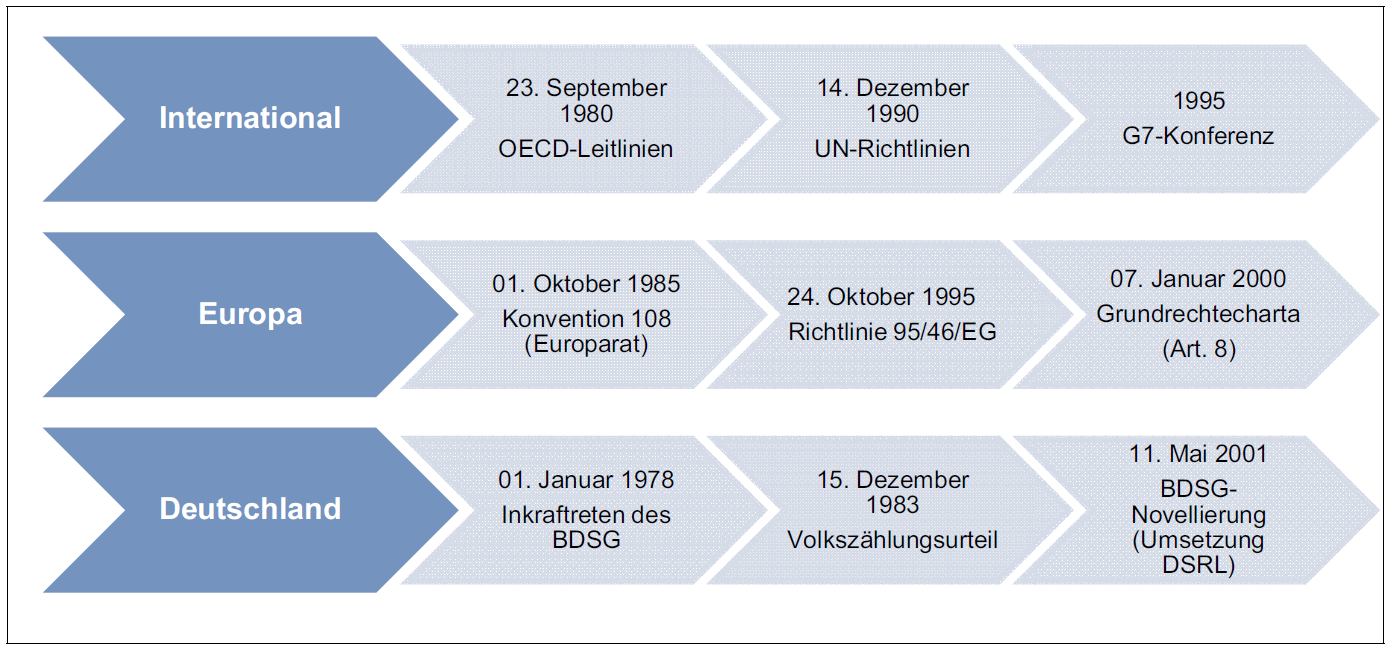
\includegraphics[scale=0.3]{datenschutz.png}
\end{center}
\caption{Entwicklung des Datenschutzes (in \cite{europData} gefunden)}
\label{pic:datenschutz}
\end{figure}
\end{frame}

\begin{frame}{Richtlinie 95/46/EG}
\begin{itemize}
	\item Richtlinie der Europäischen Gemeinschaft
	\item 1995 erlassen
	\item Schutz der Privatsphäre von natürlichen Personen bei der Verarbeitung von personenbezogenen Daten
	\item Drittstaatenregelung
\end{itemize}
\end{frame}



\begin{frame}{Weltweiter Stand des Datenschutzes}
\begin{figure}[h]
\begin{center}
	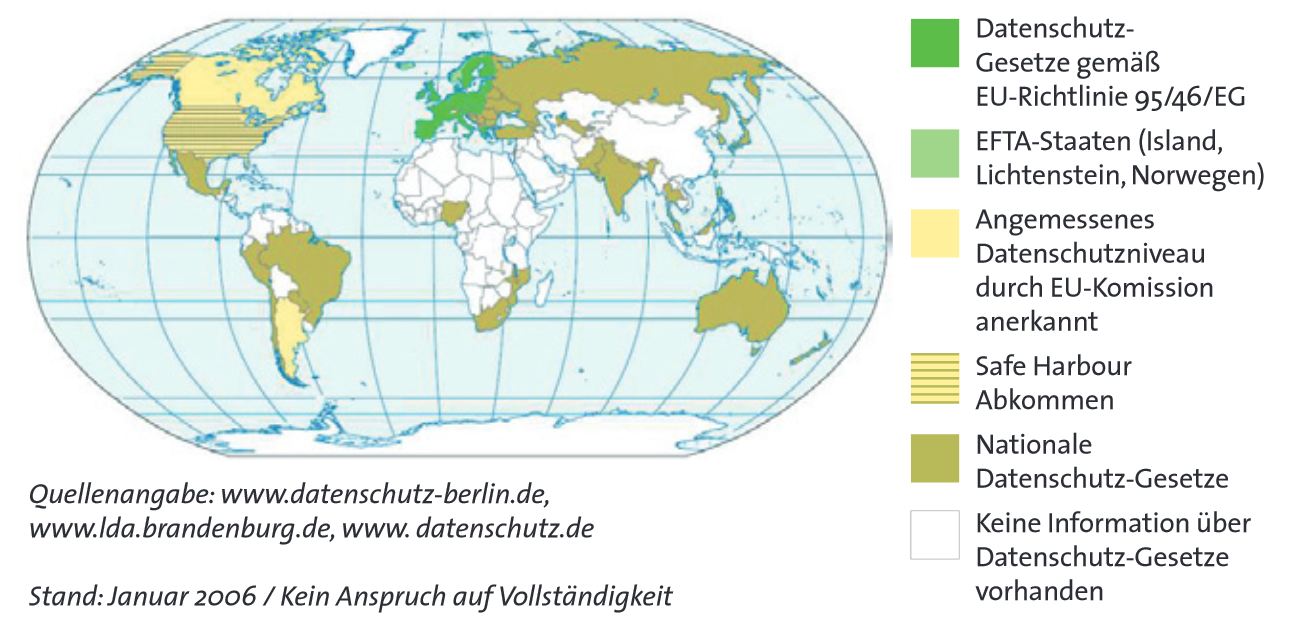
\includegraphics[scale=0.3]{datenschutzstand.png}
\end{center}
\caption{Einschätzung des weltweiten Standes zum Thema Datenschutz}
\label{pic:datenschutz}
\end{figure}
\end{frame}

\subsection{Safe harbor Abkommen}
\begin{frame}{}

\end{frame}

\section{Chancen des Datenschutzes}
\begin{frame}{}
\end{frame}


\subsection{Datenschutzgrundverordnung}
\begin{frame}{}

\end{frame}


\section*{Quellen}
\setbeamertemplate{bibliography item}{\insertbiblabel}
\setbeamercolor{bibliography item}{parent=palette primary}
\setbeamercolor*{bibliography entry title}{parent=palette primary}
\begin{frame}[shrink=10]{Quellen}
\bibliographystyle{alpha}
\bibliography{literature} 
\end{frame}

\end{document}
